
\section{Fluorescence}

It is possible that an atom which has been excited by absorbing a photon will not return to its initial state by emitting a photon of the same energy, but will instead go to an interim state for a time and emit a photon of lower energy than the photon which was originally absorbed.

This ability to seemingly change the wavelength of light (absorbing at one wavelength and emitting light of another wavelength) was known about and studied long before quantum theory was developed.  If the light is emitted rapidly following absorption, the process is called \emph{fluorescence},\marginnote{George Gabriel Stokes coined this term in his 1852 paper on the ``Refrangibility'' (wavelength change) of light, after studying extensively the ability of fluorspar and uranium glass to change invisible light beyond the violet end of the visible spectrum into blue light. He wrote ``I am almost inclined to coin a word, and call the appearance fluorescence, from fluor-spar [i.e.\ fluorite]''.} whereas if there is an appreciable delay (in some cases seconds, minutes or even many hours) it is called \emph{phosphorescence}.

The most striking examples of fluorescence occur when the absorbed radiation is in the ultraviolet region of the spectrum, and thus invisible to the human eye, and the emitted light is in the visible region.  Any number of commonplace materials (e.g.\ detergents, organic dyes, tonic water, and tooth enamel) will emit characteristic visible photons so that they appear to glow under ultraviolet illumination.

\begin{figure}
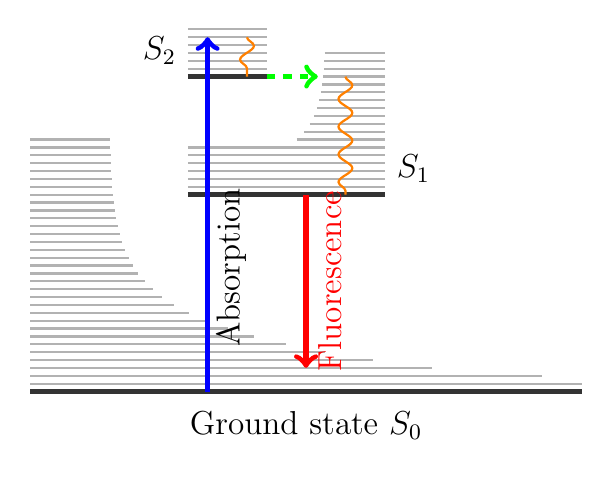
\begin{tikzpicture}[scale=0.5]

    % styles
    \tikzstyle{elec} = [line width=2pt,draw=black!80]
    \tikzstyle{vib} = [thick,draw=black!30]
    \tikzstyle{trans} = [line width=2pt,->]
    \tikzstyle{transCI} = [trans,dashed,draw=green]
    \tikzstyle{relax} = [draw=orange,thick,decorate,decoration=snake]
    \tikzstyle{rv} = [rotate=90,text=orange,pos=0.5,yshift=3mm]

    % fundamental
    \path[elec] (0,0)  -- ++ (14,0)
        node[below,pos=0.5,yshift=-1mm] {\large Ground state $S_0$};
    \path[vib] (0,0.2) -- ++ (14,0);
    \path[vib] (0,0.4) -- ++ (13,0);
    \foreach \i in {1,2,...,30} {
        \path[vib] (0,0.4 + \i*0.2) -- ++ ({2 + 10*exp(-0.2*\i)},0);
    }

    % S1
    \path[elec] (4,5) -- ++ (5,0)node[anchor=south west] {\large $S_1$};
    \foreach \i in {1,2,...,6} {
        \path[vib] (4,5 + \i*0.2) -- ++ (5,0);
    }
    \foreach \i in {1,2,...,12} {
        \path[vib] ({7.5 - 1*exp(-0.3*\i)},6.2+\i*0.2) -- (9,6.2+\i*0.2);
    }

    % S2
    \path[elec] (4,8) node[anchor=south east] {\large $S_2$} -- ++ (2,0);
    \foreach \i in {1,2,...,6} {
        \path[vib] (4,8 + \i*0.2) -- ++ (2,0);
    }

    % absorption
    \path[trans,draw=blue] (4.5,0) -- ++(0,9)
        node[rotate=90,pos=0.35,text=black,yshift=-3mm] {\large Absorption};

    % fluo
        \path[trans,draw=red](7,5) -- ++(0,-4.4)
        node[rotate=90,pos=0.5,text=red,yshift=-3mm] {\large Fluorescence};
        
        %IC
        \path[transCI] (6,8) -- ++(1.3,0);

    % relaxation vib
    \path[relax] (5.5,9.0) -- ++(0,-1.0);
    \path[relax] (8,8)     -- ++(0,-3);
\end{tikzpicture}
\caption{A Jablonski diagram showing fluorescence occuring via the closely spaced energy levels in a molecule.}
\end{figure}

There is widespread commercial use of fluorescent substances, for example in washing powders and paper to `whiten' (making white bluer makes it appear a crisper, whiter white).  Highlighter ink is often fluorescent due to the presence of pyranine.  Banknotes, postage stamps and credit cards also often have fluorescent security features.

\subsection{Fluorescent tube}
The common fluorescent lamp relies on fluorescence to convert the invisible ultraviolet radiation emitted by a mercury discharge tube into visible light.  The inside of the glass of the discharge tube is coated with fluorescent phosphors which absorbs ultraviolet and re-emits visible light.

The low pressure mercury within the tube of a fluorescent lamp has an emission spectrum (the emission is caused by electrons hitting the gaseous mercury atoms when electricity is passed through the tube) which is dominated by a line in the ultraviolet at \SI{254}{nm}, which is converted into visible emissions at many different wavelengths in the visible spectrum by the phosphors.

\begin{figure}
  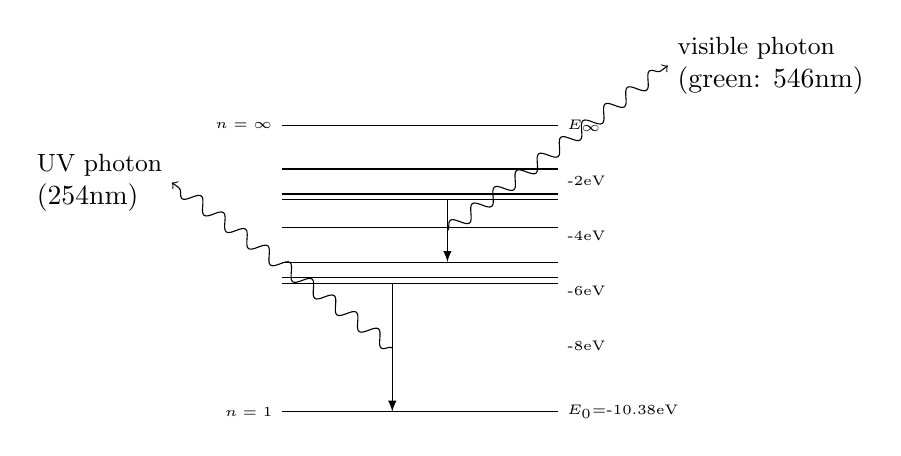
\begin{tikzpicture}[scale=0.35]
  %\draw (0,0) -- (6,0);
  \foreach \i in {-1.56,-1.57,-2.48,-2.68,-3.71,-4.95,-5.52,-5.74}{
  \draw  (0,\i) -- (10,\i);
  }
  \draw  (0,-10.38)node[left] {\tiny$n=1$} -- (10,-10.38)node[right]{\tiny$E_{0}$=\SI{-10.38}{eV}};
  \draw  (0,0)node[left] {\tiny$n=\infty$} -- (10,0)node[right]{\tiny$E_{\infty}$};
  \draw  (10,-2) node[right]{\tiny\SI{-2}{eV}};
  \draw  (10,-4) node[right]{\tiny\SI{-4}{eV}};
  \draw  (10,-6) node[right]{\tiny\SI{-6}{eV}};
  \draw  (10,-8) node[right]{\tiny\SI{-8}{eV}};
  %UV photon
  \draw[>=latex,->] (4,-5.74) --(4,-10.38);
  \draw[decorate, decoration={snake},->] (4,-8.06)--++(-8,6)node[left,align=left]{\small UV photon\\(\SI{254}{nm})};
  %Vis photon
  \draw[>=latex,->] (6,-2.68) --(6,-4.95);
  \draw[decorate, decoration={snake},->] (6,-3.82)--++(8,6)node[right,align=left]{\small visible photon\\(green: \SI{546}{nm})};
  \end{tikzpicture}
\caption{Energy levels within the mercury atom.  Two transitions, giving rise to a visible and a UV photon respectively, are shown.}
\end{figure}

Mercury also emits visible light at wavelengths of \SI{436}{nm} (blue), \SI{546}{nm} (green), and \SI{579}{nm} (yellow-orange).  These three lines can be observed superimposed on the white continuous spectrum by using a spectroscope, or even when looking at the spectrum diffracted from a CD.

\begin{marginfigure}
\includegraphics[width=\textwidth]{img/cfl.jpg}
\caption{Part of the line spectrum of a compact fluorescent tube, viewed via a diffraction grating spectrometer at Bishop Heber High School.}
\end{marginfigure}

Fluorescent lighting is more energy-efficient than old-fashioned incandescent bulbs (in which most of the input power gets turned into heat, not light).  A fluorescent tube can produce an equal amount of light using one quarter of the power of a filament bulb.  However, the uneven spectrum of traditional fluorescent lamps may cause certain colors to appear different than when illuminated by incandescent light or daylight.


